\documentclass[11pt,class=report,crop=false]{standalone}
\usepackage[screen]{../python}


\begin{document}


%====================================================================
\chapitre{Nombres complexes I}
%====================================================================

\objectifs{Nous allons faire des calculs avec les nombres complexes. Ce sera facile car  \Python{} sait les manipuler.}

\index{nombre complexe}

%%%%%%%%%%%%%%%%%%%%%%%%%%%%%%%%%%%%%%%%%%%%%%%%%%%%%%%%%%%%%%%%
%%%%%%%%%%%%%%%%%%%%%%%%%%%%%%%%%%%%%%%%%%%%%%%%%%%%%%%%%%%%%%%%

\begin{cours}[Nombres complexes]

Avec \Python, tu manipules les nombres complexes comme les autres nombres.
La notation pour le nombre complexe $i$ (qui vérifie $i^2=-1$) est le symbole \ci{j} (plus exactement \ci{1j}).
Par exemple, le nombre complexe $4-3i$ se note \ci{4-3j}. 
Ensuite les opérations classiques s'écrivent comme d'habitude : par exemple le calcul $(1+2i)(4-i)$ s'écrit \ci{(1+2j)*(4-1j)} et \Python{} renvoie \ci{6+7j}.

\begin{itemize}
  \item Addition $z_1+z_2$ : \ci{z1 + z2}
  \item Multiplication $z_1 \cdot z_2$ : \ci{z1 * z2}
  \item Puissance $z^n$ : \ci{z1 ** n}
  \item Inverse $\frac{1}{z}$ : \ci{1/z}
  \item Partie réelle $a$ de $z=a+ib$ : \ci{z.real}\index{real@\ci{real}} \quad (sans parenthèses)
  \item Partie imaginaire $b$ de $z=a+ib$ : \ci{z.imag}\index{imag@\ci{imag}} \quad (sans parenthèses) 
  \item Module $|z| = \sqrt{a^2+b^2}$ : \ci{abs(z)}\index{abs@\ci{abs}}
  \item Conjugué $\bar z = a-ib$ : \ci{z.conjugate()}\index{conjugate@\ci{conjugate}}
\end{itemize}

\bigskip

Bien sûr \Python{} ne fait pas toujours des calculs exacts (par exemple, lors d'une division ou pour le calcul d'un module), car les nombres sont des nombres complexes flottants.
\end{cours}


%%%%%%%%%%%%%%%%%%%%%%%%%%%%%%%%%%%%%%%%%%%%%%%%%%%%%%%%%%%%%%%%
% Activité 1
%%%%%%%%%%%%%%%%%%%%%%%%%%%%%%%%%%%%%%%%%%%%%%%%%%%%%%%%%%%%%%%%

\begin{activite}[Manipuler les nombres complexes]

\objectifs{Objectifs : faire des calculs avec les nombres complexes.}

\begin{enumerate}
  \item Définis les nombres complexes $z_1 = 1+2i$ et $z_2=3-i$.
  Demande à la machine de calculer :
  $$z_1+z_2 \qquad z_1z_2 \qquad z_1^2 \qquad |z_1| \qquad \frac{1}{z_1} $$
    
  \item Définis le nombre complexe $z = (3-4i)^2(2+i)$. 
  Calcule à la machine la partie réelle de $z$, sa partie imaginaire et son conjugué.
  
  \item Définis tes propres fonctions pour les opérations sur les nombres complexes.  Représente le nombre complexe $z=a+i b$ par le couple de réels $(a,b)$ et $z' =a'+i b'$ par le couple de réels $(a',b')$ (tu n'as pas le droit d'utiliser les nombres complexes de \Python).
  
  \begin{itemize}
    \item Programme une fonction \ci{addition(a,b,aa,bb)} 
    qui renvoie le couple de réels correspondant au résultat de $(a+i b) + (a'+i b')$.
    \item Programme une fonction \ci{multiplication(a,b,aa,bb)} 
    qui renvoie le couple de réels correspondant au résultat de $(a+i b) \times (a'+i b')$.   
    
    \item  Programme une fonction \ci{conjugue(a,b)}
    qui renvoie le couple de réels correspondant au conjugué de 
    $a+i b$.
    
    \item  Programme une fonction \ci{module(a,b)}
    qui renvoie le module de $a+i b$ (c'est un nombre réel).    
    
    \item  Programme une fonction \ci{inverse(a,b)}
    qui pour $z= a+i b$ teste d'abord si $z$ n'est pas nul et dans ce cas renvoie le couple de réels associé à l'inverse de $z$ en utilisant une des formules :
$$\frac{1}{z} = \frac{\bar z}{|z|^2} \qquad \text{ ou } \qquad \frac{1}{z} = \frac{a-ib}{a^2+b^2}.$$
    
    \item  Programme une fonction \ci{puissance(a,b,n)}
    qui pour $z= a+i b$ et $n\ge0$, renvoie le couple de réels associé à $z^n$. (\emph{Indications.} Par définition $z^0 = 1$. On pourra construire une boucle et utiliser une des fonctions précédentes.)
    
\end{itemize}    
  
\end{enumerate} 
\end{activite}

%%%%%%%%%%%%%%%%%%%%%%%%%%%%%%%%%%%%%%%%%%%%%%%%%%%%%%%%%%%%%%%%
%%%%%%%%%%%%%%%%%%%%%%%%%%%%%%%%%%%%%%%%%%%%%%%%%%%%%%%%%%%%%%%%

\begin{cours}[Rappels Matplotlib]

\index{module!matplotlib@\ci{matplolib}}

Voici comment afficher des points de coordonnées $(x,y)$ et un segment à l'aide du module \ci{matplotlib}.

\begin{center}
\begin{minipage}{0.75\textwidth}
\begin{lstlisting}
import matplotlib.pyplot as plt

plt.clf()  # Efface tout
plt.axhline(y=0, color='r', linestyle='-')  # Axe x
plt.axvline(x=0, color='r', linestyle='-')  # Axe y
plt.axes().set_aspect('equal')  # Repère orthonormé

x1 = 1
y1 = 2
plt.scatter(x1,y1,color='red',s=80)     # Un premier point

x2 = 5
y2 = 3
plt.scatter(x2,y2,color='blue',s=80)    # Un second point

# Un segment reliant les points
plt.plot([x1,x2],[y1,y2],color='green')  

plt.show()  # Lancement de la fenêtre
\end{lstlisting} 
\end{minipage}
\end{center}

\begin{center}
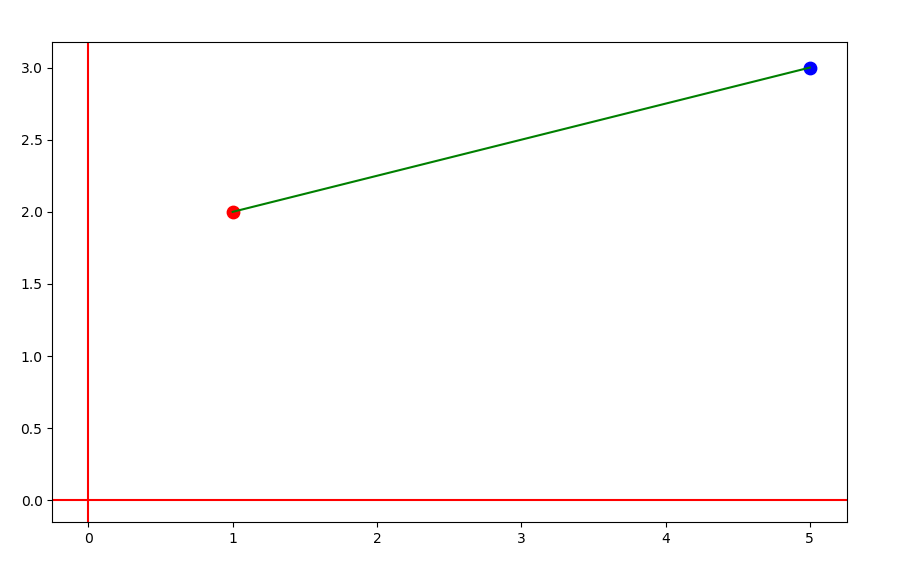
\includegraphics[scale=\myscale,scale=0.4]{ecran-complexes1-cours}
\end{center}	 

\end{cours}

%%%%%%%%%%%%%%%%%%%%%%%%%%%%%%%%%%%%%%%%%%%%%%%%%%%%%%%%%%%%%%%%
% Activité 2 - Visualisation
%%%%%%%%%%%%%%%%%%%%%%%%%%%%%%%%%%%%%%%%%%%%%%%%%%%%%%%%%%%%%%%%

\begin{activite}[Visualiser les nombres complexes]

\objectifs{Objectifs : afficher un point connaissant son affixe $z$.}

\begin{enumerate}
  \item Dessine le point d'affixe $1$ et celui d'affixe $i$.
  Pour un nombre complexe $z$, par exemple $z = -2+3i$, dessine le point d'affixe $z$.
   
  \item Pour un nombre complexe $z$, par exemple $z = 3-2i$, dessine les points d'affixes :
  $$z \qquad 2z \qquad iz \qquad \bar z \qquad \frac{z^2}{|z|} \qquad \frac{1}{z}$$
  
  \item 
  \begin{itemize}
    \item Programme une fonction \ci{affiche_triangle(z1,z2,z3)} qui trace le triangle dont les sommets ont pour affixes $z_1$, $z_2$, $z_3$.
 
   \smallskip 
   
\begin{center}
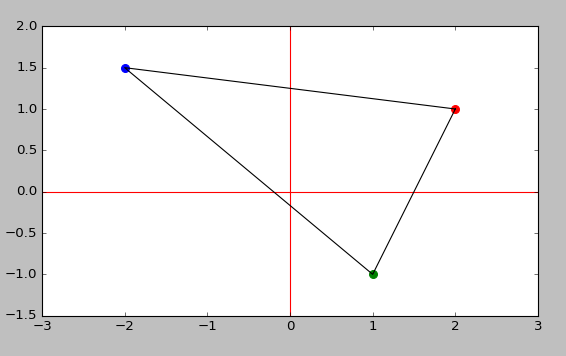
\includegraphics[scale=\myscale,scale=0.5]{ecran-complexes1-3}
\end{center}	 
    
    \item On fixe $z \in \Cc$. 
  Quelle semble être la nature du triangle 
déterminé par $z$, $2z$, $(1+2i)z$ ?   
    
    \item On pose $\omega = -\frac12+\frac{\sqrt3}{2}i$. On fixe $z \in \Cc$.
    Quelle semble être la nature du triangle donné par $z$, $\omega z$, $\omega^2 z$ ? 
\end{itemize}    
  
\end{enumerate} 
\end{activite}



%%%%%%%%%%%%%%%%%%%%%%%%%%%%%%%%%%%%%%%%%%%%%%%%%%%%%%%%%%%%%%%%
% Activité 3 - 
%%%%%%%%%%%%%%%%%%%%%%%%%%%%%%%%%%%%%%%%%%%%%%%%%%%%%%%%%%%%%%%%

\begin{activite}[Résolution d'une équation linéaire]

\objectifs{Objectifs : résoudre des équations linéaires en utilisant les nombres complexes. Ici nous allons \og{}hacker\fg{} les nombres complexes. En informatique un \og{}hack\fg{} est un détournement d'une fonctionnalité.}

\bigskip

\textbf{Résolution.}
Tu vas programmer une fonction \ci{solution_equation_lineaire(equation)}
qui calcule et renvoie la solution d'une équation linéaire. 
L'équation est donnée en paramètre sous la forme d'une chaîne de caractères. Par exemple
avec \ci{"7*x+3 = 0"}, la fonction renvoie \ci{-0.42857...} comme valeur approchée 
de $-\frac37$.
Autre exemple avec : \ci{"3*(x+1) + x = 2*x+1"}, la fonction renvoie \ci{-1.0}.

Attention : il faut explicitement écrire les multiplications avec le caractère \og{}\ci{*}\fg{}.


\bigskip

\textbf{Astuce.}
L'idée est la suivante, une équation linéaire se ramène à la forme :
$$a + bx = 0$$
dont une solution est $-\frac{a}{b}$.
L'astuce est de remplacer chaque \og{}$x$\fg{} de l'équation par le nombre complexe $i$. On obtient ainsi un nombre complexe $a+ib$. En extrayant la partie réelle et la partie imaginaire, on renvoie la solution (réelle) $-a/b$.

\bigskip

\textbf{Exemple simple.}
Partant de l'équation $7x+3 = 0$, on ne garde que la partie gauche de l'équation $7x+3$. On remplace la lettre $x$ par le nombre complexe $i$, on obtient 
$7i+3$. On extrait sa partie réelle $a=3$ et sa partie imaginaire $b=7$. On renvoie la solution $-a/b = -\frac37$.

\bigskip

\textbf{Exemple compliqué.}
Soit l'équation $3(x+1) + x = 2x+1$. Il faut d'abord tout basculer à gauche du signe égal afin de se ramener à l'équation $3(x+1) + x - \big(2x+1 \big) = 0$.
On ne garde que l'expression à gauche du signe égal : 
$3(x+1) + x - \big(2x+1 \big)$.
On remplace ensuite la variable $x$ par le nombre complexe $i$.
L'expression devient un nombre complexe $3(i+1) + i - \big(2i+1 \big)$.
On note $z$ ce nombre complexe, on calcule sa partie réelle $a = 2$  et sa partie imaginaire $b = 2$. On calcule $-a/b = -1$. La solution de notre équation est donc $x = -1$.


\bigskip

% \textbf{Algorithme.}

  \begin{algorithme}
  \sauteligne 
  \begin{itemize}
    \item 
    \begin{itemize}
     \item Entrée : une chaîne de caractères représentant une équation linéaire en $x$.
     \item Sortie : la valeur numérique de la solution $x$.
     \end{itemize}  
     
   \item Soient \ci{G} et \ci{D} les deux chaînes de part et d'autre du signe \og{}=\fg{}. (Utilise
   \ci{equation.split("=")}.)
   
   \index{chaine@chaîne de caractères!split@\ci{split}}
   \index{split@\ci{split}}
   
   \item Former la chaîne correspondant à la partie gauche moins la partie droite :  
   \ci{G + "-(" + D + ")"}.
   
   \item Pour remplacer $x$ par $i$, il faut remplacer le caractère \ci{"x"} par la chaîne \ci{"1j"}. (Utilise \ci{chaine.replace(mot,nouv_mot)}.) On obtient ainsi une chaîne \ci{z_str}.
  
  \index{replace@\ci{replace}}
  \index{chaine@chaîne de caractères!replace@\ci{replace}}
  	
  \item Transformer la chaîne en un nombre complexe par l'opération :
  \mycenterline{\ci{z = eval(z_str)}}
  
  \index{eval@\ci{eval}}
  \index{chaine@chaîne de caractères!eval@\ci{eval}}
  
  \item Calculer la partie réelle \ci{a} et la partie imaginaire \ci{b} de \ci{z}.
  
  \item Renvoyer \ci{-a/b}.
   
 \end{itemize}  
 \end{algorithme}


\end{activite}

%%%%%%%%%%%%%%%%%%%%%%%%%%%%%%%%%%%%%%%%%%%%%%%%%%%%%%%%%%%%%%%%
%%%%%%%%%%%%%%%%%%%%%%%%%%%%%%%%%%%%%%%%%%%%%%%%%%%%%%%%%%%%%%%%

\begin{cours}[\'Equation du second degré]

\index{equation du second degre@équation du second degré}

Soit $a,b,c \in \Rr$ avec $a \neq 0$. On considère l'équation 
$$az^2+bz+c=0.$$
On note $\Delta = b^2-4ac$. Selon le signe de $\Delta$ les solutions sont les suivantes :
\begin{itemize}
  \item $\Delta > 0$ : deux solutions réelles \quad $z_1 = \dfrac{-b+\sqrt{\Delta}}{2a}$  \  et \  $z_2 = \dfrac{-b-\sqrt{\Delta}}{2a}$.
  \item $\Delta = 0$ : solution double \quad $z_0 = \dfrac{-b}{2a}$.
  \item $\Delta < 0$ : deux solutions complexes \quad $z_1 = \dfrac{-b+i\sqrt{|\Delta|}}{2a}$ \  et \  $z_2 = \dfrac{-b-i\sqrt{|\Delta|}}{2a}$.
\end{itemize}
\end{cours}

%%%%%%%%%%%%%%%%%%%%%%%%%%%%%%%%%%%%%%%%%%%%%%%%%%%%%%%%%%%%%%%%
% Activité 4
%%%%%%%%%%%%%%%%%%%%%%%%%%%%%%%%%%%%%%%%%%%%%%%%%%%%%%%%%%%%%%%%

\begin{activite}[\'Equation du second degré]
	

\objectifs{Objectifs : résoudre les équations du second degré, y compris lorsque le discriminant est négatif.}

On considère l'équation :
$$az^2+bz+c=0 \qquad \text{ avec } \quad a,b,c \in \Rr \quad \text{ et } \quad a \neq 0.$$
\begin{enumerate}
  \item \textbf{\'Equation du second degré.}
  Programme une fonction \ci{solution_trinome(a,b,c)} qui renvoie les solutions de l'équation sous la forme d'une liste de deux nombres \ci{[z1,z2]} (si la solution est double, renvoie la liste \ci{[z0,z0]}).
  
  
  Exemple. Calcule les solutions de :
  $$z^2 - 2z + 1 = 0 \qquad  z^2 + z - 1 = 0 \qquad z^2 + z + 1 = 0$$
  
  \item \textbf{Somme et produit.} 
  Lorsque l'on connaît la somme $S$ et le produit $P$ de deux nombres $z_1$ et $z_2$,
  on peut retrouver $z_1$ et $z_2$. Comment faire ? Réponse : $z_1$ et $z_2$ sont les solutions de l'équation :
  $$z^2 - S z + P = 0.$$
  Programme une fonction \ci{solution_somme_produit(S,P)} qui renvoie la liste \ci{[z1,z2]} des solutions.
  
  Exemple. Trouve deux nombres dont la somme est $10$ et le produit est $20$.
  
  \item \textbf{\'Equation bicarrée.}
  Une équation bicarrée est de la forme :
  $$ax^4 + bx^2 + c = 0.$$
  Nous étudions seulement les cas où $\Delta = b^2 -4ac \ge 0$, pour lesquels l'équation admet $4$ solutions (réelles ou complexes).
  
  On commence par poser $X=x^2$ et résoudre l'équation du second degré :
  $$ aX^2 + bX + c = 0.$$
  Cette dernière équation admet deux solutions réelles $X_1$ et $X_2$.
  Pour chacune de ces solutions $X$ :
    \begin{itemize}
      \item si $X \ge 0$, on obtient deux solutions, $+\sqrt{X}$ et $-\sqrt{X}$ ;
      \item si $X < 0$, on obtient deux solutions, $+i\sqrt{-X}$ et $-i\sqrt{-X}$.
    \end{itemize}
   On obtient ainsi $4$ solutions ($2$ associées à $X_1$ et $2$ associées à $X_2$).
   
   Programme une fonction \ci{solution_bicarre(a,b,c)} qui renvoie les $4$ solutions    
    de l'équation  $ax^4 + bx^2 + c = 0$ après avoir vérifié que $\Delta = b^2 -4ac \ge 0$.
  
  Exemple. Trouve les $4$ solutions de l'équation $x^4-2x^2-3=0$.  
\end{enumerate} 
\end{activite}



%%%%%%%%%%%%%%%%%%%%%%%%%%%%%%%%%%%%%%%%%%%%%%%%%%%%%%%%%%%%%%%%
% Activité 5
%%%%%%%%%%%%%%%%%%%%%%%%%%%%%%%%%%%%%%%%%%%%%%%%%%%%%%%%%%%%%%%%

\begin{activite}[Famille de racines]

\objectifs{Objectifs : afficher les solutions d'une famille d'équations du second degré.}

\begin{enumerate}
  \item \textbf{Afficher les racines.}
  Programme une fonction \ci{affiche_racines(a,b,c)} qui affiche les deux points correspondant aux deux solutions de l'équation $ax^2+bx+c=0$.
  
  \emph{Amélioration.} C'est mieux d'autoriser en argument optionnel le choix de la couleur du point par une entête \ci{affiche_racines(a,b,c,couleur='red')}.
  
  
\emph{Retrouve sur la figure ci-dessous les racines des polynômes}
$x^2 - 2x + 1 = 0$,  $x^2 + x - 1 = 0$ et $x^2 + x + 1 = 0$.
\begin{center}
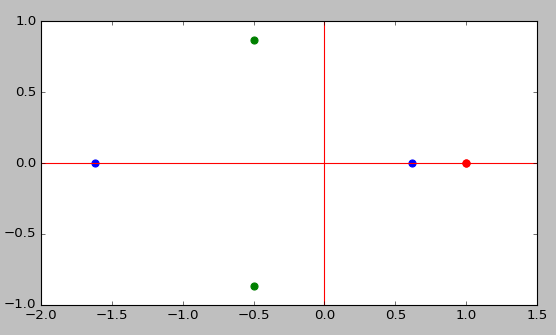
\includegraphics[scale=\myscale,scale=0.4]{ecran-complexes1-5a}
\end{center}	 
  
  
  \item \textbf{Famille de racines.}
  On considère deux polynômes
  $$P_0(x) = x^2 + b_0 x + c_0 \quad \text{ avec } \quad \Delta_0 = b_0^2-4c_0 \le 0,$$
  $$P_1(x) = x^2 + b_1 x + c_1 \quad \text{ avec } \quad \Delta_1 = b_1^2-4c_1 \le 0.$$  
  On définit pour $0 \le t \le 1$ :
  $$P_t(x) = (1-t)P_0(x) + tP_1(x) = x^2 + \big((1-t)b_0 + tb_1\big) x + (1-t)c_0 + tc_1.$$
  
  \emph{Question.} Quelle forme a l'ensemble des racines de la famille 
  $\{P_t(x)\}_{0 \le t \le 1}$ ?
  
  Programme une fonction \ci{affiche_famille(b0,c0,b1,c1)} :
  \begin{itemize}
    \item qui affiche les solutions de $P_0(x)=0$ (en rouge par exemple),
    \item qui affiche les solutions de $P_1(x)=0$ (en vert par exemple),    
    \item qui affiche les solutions de $P_t(x)=0$ pour $n$ valeurs $t$, avec $0 \le t \le1$ (en bleu par exemple).
  \end{itemize}
  
  Pour les valeurs de $t$, tu peux les choisir de la forme $k/n$ avec $0 \le k < n$.
  
  \emph{Amélioration.} C'est mieux d'autoriser que $n$ soit un argument optionnel par une entête du type  \ci{affiche_famille(b0,c0,b1,c1,n=100)}.
  
  
  
\emph{Exemple ci-dessous $P_0(x) = x^2-2x+2$ et $P_1(x) = x^2+3x+\frac{12}{5}$, avec seulement $n=3$ points \couleurnb{bleus }{}intermédiaires. Pour répondre à la question il faut afficher plus de points intermédiaires.}
\begin{center}
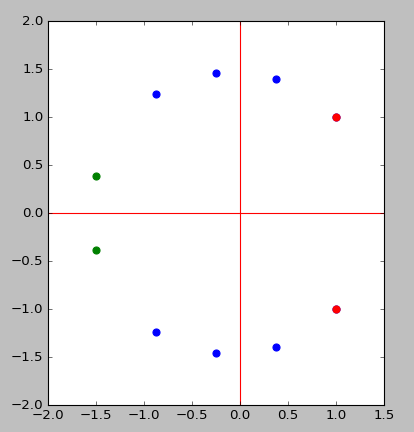
\includegraphics[scale=\myscale,scale=0.5]{ecran-complexes1-5b}
\end{center}	 

\end{enumerate} 
\end{activite}

\end{document}
